\documentclass[english]{article}

%% Packages pull in extra commands:
%% http://en.wikibooks.org/wiki/LaTeX/Packages

\usepackage{hyperref}
%%\usepackage[latin9]{inputenc}
\usepackage[letterpaper]{geometry}
\geometry{verbose,tmargin=1in,bmargin=1in,lmargin=1in,rmargin=1in}
\usepackage{amsmath}
\usepackage{amssymb}
\usepackage{graphicx}
\usepackage{float}
\usepackage{array}
\usepackage{tikz}

% New commands serve as shorthand for frequently used command combinations.
\newcommand{\ind}[1]{\mathbf{1}\left(#1\right)}
\newcommand{\bx}{\mathbf{x}}
\newcommand{\E}{\mathbf{E}}

\title{CIS 520, Machine Learning, Fall 2018: Assignment 1}
\author{Wentao He}

\begin{document}
\maketitle

{\normalsize \noindent Collaborators: \underline{N/A}} \\


\section{Conditional independence in probability models}

\begin{enumerate}
\item We can write $p(x_i)$ as:
  \begin{align*}
    p(x_i) = &\;\sum_{j=1}^{k} p(x_i \mid z_i=j)\pi_j \\
    = &\; \sum_{j=1}^{k} f_j(x_i)\pi_j
  \end{align*}

\item The formula for $p(x_1, \dots, x_n)$ is:
  \begin{align*}
    p(x_1, \dots, x_n) = &\; \sum_{z_1, \dots, z_n} p(x_1, \dots, x_n \mid z_1, \dots, z_n) \\
    =&\; \sum_{z_1, \dots, z_n} p(x_1 \mid x_2, \dots, x_n, z_1, \dots, z_n) \dots p(x_n \mid z_1, \dots, z_n)p(z_1, \dots, z_n) \\
    =&\; \sum_{z_1, \dots, z_n} \prod_{i=1}^{n} p(x_i \mid z_i)p(z_i) \\
    =&\; \prod_{i=1}^{n} \sum_{j=1}^{k} p(x_1 \mid z_i\,=j\,)\pi_j \\
    =&\; \prod_{i=1}^{n} \sum_{j=1}^{k} f_j(x_i)\pi_j
  \end{align*}

\item The formula for $p(z_u = v \mid x_1, \dots, x_n)$ is:
  \begin{align*}
    p(z_u = v \mid x_1, \dots, x_n) = &\; \dfrac{p(x_1, \dots, x_n \mid z_u)p(z_u=v)}{p(x_1, \dots, x_n} \\
    =&\; \dfrac{p(x_u \mid z_u=v) \pi_v \prod_{i=1,i \neq u}^{n} \sum_{j=1}^{k} p(x_i \mid z_i=j) \pi_j}{\prod_{i=1}^{n} \sum_{j=1}^{k} p(x_1 \mid z_i=j) \pi_j} \\
    =&\; \dfrac{p(x_u \mid z_u = v) \pi_v}{\sum_{j=1}^{k} p(x_u \mid z_u = j) \pi_j} \\
    =&\; \dfrac{f_v(x_u)\pi_v}{\sum_{j=1}^{k} f_j(x_u)\pi_j}
  \end{align*}
\end{enumerate}

\section{Non-Normal Norms}

\begin{enumerate}
\item

For the given vectors,the point closest to $x_1$ under each of the following norms is \\\\
a) $L_0$: $x_4$ with distance = 2 \\
b) $L_1$: $x_3$ with distance = 1.2 \\
c) $L_2$: $x_2$ with distance = 0.79 \\
d) $L_{\inf}$: $x_2$ with distance = 0.6 \\

\item

Draw the 1-Nearest Neighbor decision boundaries with the given norms and lightly shade the o region: \\ \\ a) $L_0$ \qquad \qquad \qquad \qquad \qquad \qquad \qquad \qquad b) $L_1$\\ 
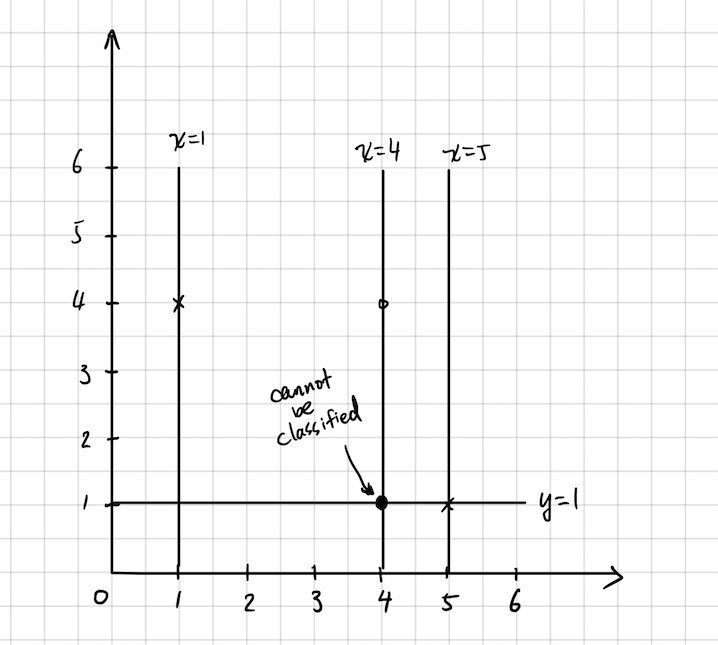
\includegraphics[width=0.4\textwidth]{images/L0.png}
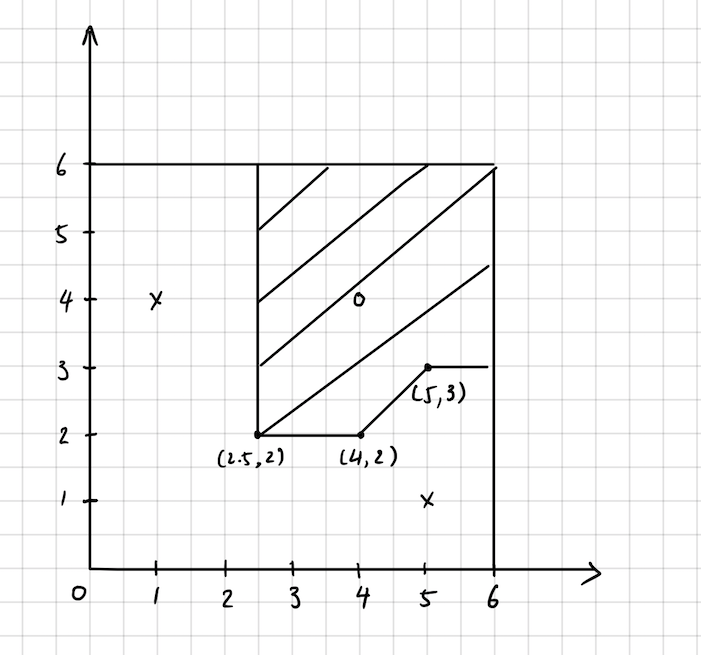
\includegraphics[width=0.4\textwidth]{images/L1.png} \\
c) $L_2$ \qquad \qquad \qquad \qquad \qquad \qquad \qquad \qquad d) $L_{\inf}$\\
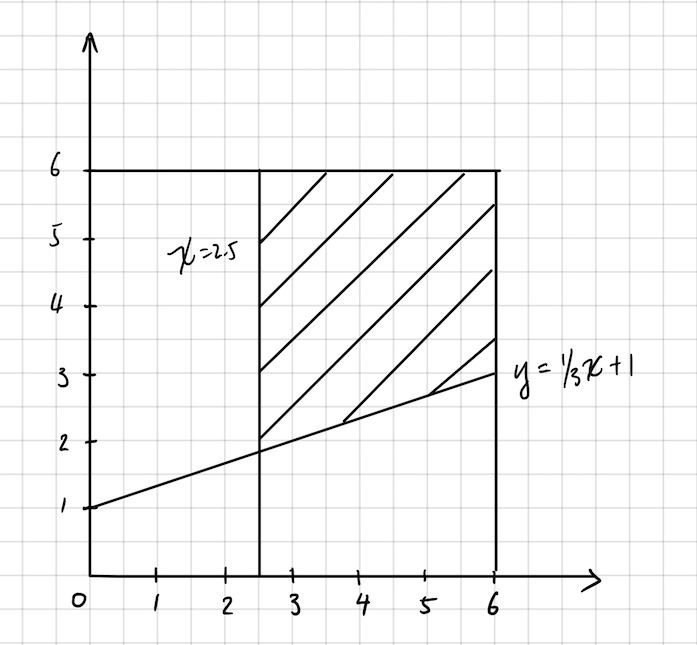
\includegraphics[width=0.4\textwidth]{images/L2.png}
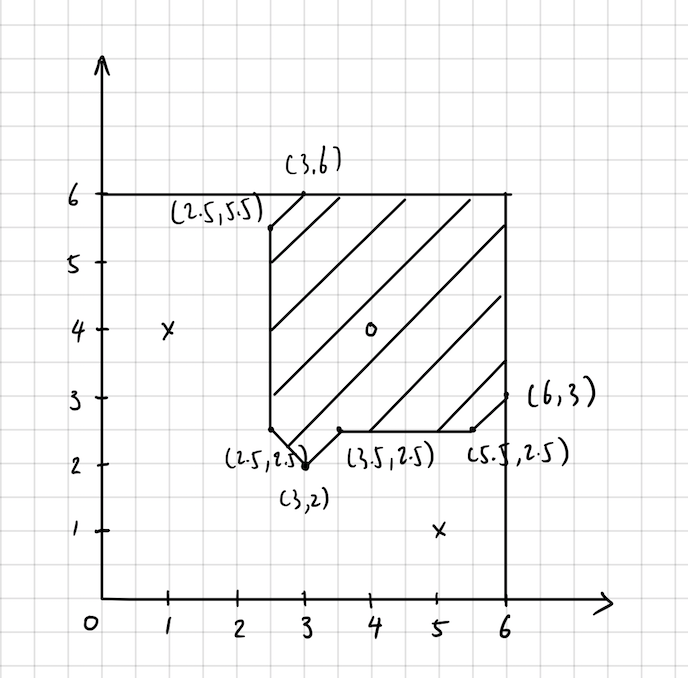
\includegraphics[width=0.4\textwidth]{images/Linf.png} \\

\end{enumerate}

\section{Decision trees}
\begin{enumerate}
\item Concrete sample training data.
  \begin{enumerate}
  \item The sample entropy $H(Y)$ is:
    \begin{align*}
      H(Y) =&\; - \sum_{i=1}^{k} P(Y = y_i) \log_2 P(Y = y_i) \\
      =&\; -P(Y = {+}) \log_2 P(Y = {+}) -  P(Y = {-}) \log_2 P(Y = {-})\\
      =&\; -(\dfrac{16}{30}) \log_2 (\dfrac{16}{30}) - (\dfrac{14}{30}) \log_2 (\dfrac{14}{30}) \\
      =&\; 0.9968
    \end{align*}

  \item The information gains are $IG(X_1) = \textbf{\underline{0.0114}}$ and $IG(X_2) = \textbf{\underline{0.0487}}$. \\ \\
  To find the information gains $IG(X_1)$ and $IG(X_2)$, we must first find $H(Y \mid X_1)$ and $H(Y \mid X_2)$. \\ \\
  $H(Y \mid X_1)$ can be calculated as follows:
    \begin{align*}
      H(Y \mid X_1) = &\; \sum_{x} P(X_1 = x) H(Y \mid X_1 = x) \\
      =&\; - \sum_{x} P(X_1 = x) \sum_{y} P(Y = y \mid X_1 = x) \log_2 P(Y = y \mid X_1 = x) \\
      =&\; - \sum_{x, y} P(X_1 = x, Y = y) \log_2 P(Y = y \mid X_1 = x) \\
      =&\; - P(X_1 = T, Y = +) \log_2 P(Y = + \mid X_1 = T) - P(X_1 = T, Y = -) \log_2 P(Y = - \mid X_1 = T) \\
      &\; - P(X_1 = F, Y = +) \log_2 P(Y = + \mid X_1 = F) - P(X_1 = F, Y = -) \log_2 P(Y = - \mid X_1 = F) \\
    \end{align*}
  The aforementioned probabilities can be calculated as follows: \\
    \begin{align*}
      P(X_1 = T, Y = +) =&\; \dfrac{6}{30} \\
      P(Y = + \mid X_1 = T) =&\; \dfrac{6}{13} \\
      P(X_1 = T, Y = -) =&\; \dfrac{7}{30} \\
      P(Y = - \mid X_1 = T) =&\; \dfrac{7}{13} \\
      P(X_1 = F, Y = +) =&\; \dfrac{10}{30} \\
      P(Y = + \mid X_1 = F) =&\; \dfrac{10}{17} \\
      P(X_1 = F, Y = -) =&\; \dfrac{7}{30} \\
      P(Y = - \mid X_1 = F) =&\; \dfrac{7}{17} \\
    \end{align*}
  $H(Y \mid X_1)=$ can be calculated as follows: \\
    \begin{align*}
      H(Y \mid X_1) = &\; - \dfrac{6}{30} \log_2 \dfrac{6}{13} - \dfrac{7}{30} \log_2 \dfrac{7}{13} - \dfrac{10}{30} \log_2 \dfrac{10}{17} - \dfrac{7}{30} \log_2 \dfrac{7}{17} \\
      = &\; 0.9854 \\
    \end{align*}
  Therefore:
    \begin{align*}
      IG(X_1) =&\; H(Y) - H(Y \mid X_1) \\
      =&\; 0.9968 - 0.9854 \\
      =&\; 0.0114 \\
    \end{align*}
  Similarly, $H(Y \mid X_2)$ can be calculated as follows:
    \begin{align*}
      H(Y \mid X_2) = &\; \sum_{x} P(X_2 = x) H(Y \mid X_2 = x) \\
      =&\; - \sum_{x} P(X_2 = x) \sum_{y} P(Y = y \mid X_2 = x) \log_2 P(Y = y \mid X_2 = x) \\
      =&\; - \sum_{x, y} P(X_2 = x, Y = y) \log_2 P(Y = y \mid X_2 = x) \\
      =&\; - P(X_2 = T, Y = +) \log_2 P(Y = + \mid X_2 = T) - P(X_2 = T, Y = -) \log_2 P(Y = - \mid X_2 = T) \\
      &\; - P(X_2 = F, Y = +) \log_2 P(Y = + \mid X_2 = F) - P(X_2 = F, Y = -) \log_2 P(Y = - \mid X_2 = F) \\
    \end{align*}
  The aforementioned probabilities can be calculated as follows: \\
    \begin{align*}
      P(X_2 = T, Y = +) =&\; \dfrac{4}{30} \\
      P(Y = + \mid X_2 = T) =&\; \dfrac{4}{11} \\
      P(X_2 = T, Y = -) =&\; \dfrac{7}{30} \\
      P(Y = - \mid X_1 = T) =&\; \dfrac{7}{11} \\
      P(X_2 = F, Y = +) =&\; \dfrac{12}{30} \\
      P(Y = + \mid X_2 = F) =&\; \dfrac{12}{19} \\
      P(X_2 = F, Y = -) =&\; \dfrac{7}{30} \\
      P(Y = - \mid X_2 = F) =&\; \dfrac{7}{19} \\
    \end{align*}
  $H(Y \mid X_2)=$ can be calculated as follows: \\
    \begin{align*}
      H(Y \mid X_2) = &\; - \dfrac{4}{30} \log_2 \dfrac{4}{11} - \dfrac{7}{30} \log_2 \dfrac{7}{11} - \dfrac{12}{30} \log_2 \dfrac{12}{19} - \dfrac{7}{30} \log_2 \dfrac{7}{19}\\
      = &\; 0.9481 \\
    \end{align*}
  Therefore:
    \begin{align*}
      IG(X_2) =&\; H(Y) - H(Y \mid X_2) \\
      =&\; 0.9968 - 0.9481 \\
      =&\; 0.0487 \\
    \end{align*}
  The information gains are:
    \begin{align*}
      IG(X_1) =&\; \textbf{\underline{0.0114}} \\
      IG(X_2) =&\; \textbf{\underline{0.0487}} \\
    \end{align*}
 
  \item The decision tree that would be learned is shown in Figure
    \ref{fig:decision_tree}.
    %% The [H], in combination with the float package, forces latex to
    %% generate the figure in exactly this part of the document
    %% instead of ``floating'' it to another part.
  Since $IG(X_2) > IG(X_1)$, this specific set of training example will be based on feature $X_2$:
    \begin{figure}[H]
      \centering
      \tikzstyle{dir}=[->, very thick]
      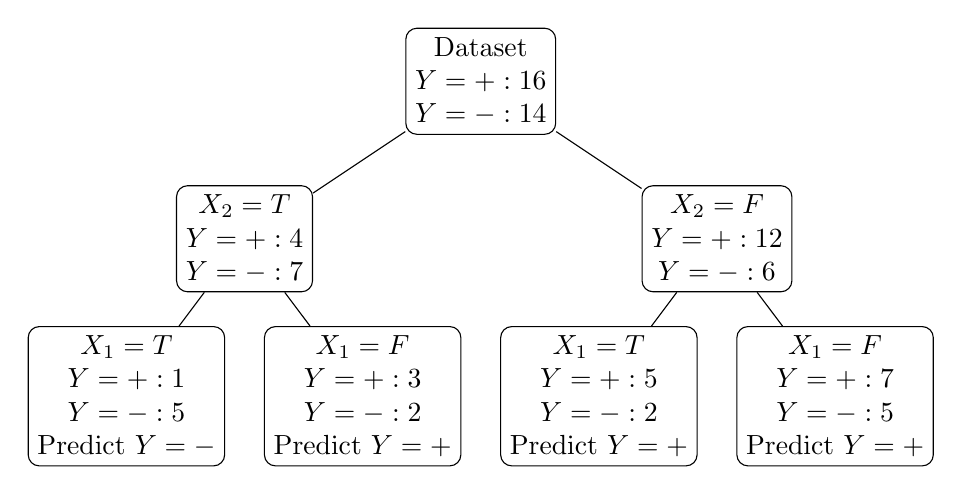
\begin{tikzpicture}[every node/.style = {shape=rectangle, rounded corners,
          draw, align=center,}]]
          \tikzstyle{level 1}=[level distance=20mm,sibling distance=60mm]
          \tikzstyle{level 2}=[level distance=20mm,sibling distance=30mm]
        \node {Dataset \\ $Y = +: 16$ \\ $Y = -:14$}
          child { node {$X_2 = T$ \\ $Y = +: 4$ \\ $Y = -:7$}
            child {node {$X_1 = T$ \\ $Y = +: 1$ \\ $Y = -:5$ \\Predict $Y = -$}}
            child {node {$X_1 = F$ \\ $Y = +: 3$ \\ $Y = -:2$ \\Predict $Y = +$}}
          }
          child { node {$X_2 = F$ \\ $Y = +: 12$ \\ $Y = -:6$}
            child {node {$X_1 = T$ \\ $Y = +: 5$ \\ $Y = -:2$ \\ Predict $Y = +$}}
            child {node {$X_1 = F$ \\ $Y = +: 7$ \\ $Y = -:5$ \\ Predict $Y = +$}}
          };
      \end{tikzpicture}
      \caption{The decision tree that would be learned.}
      \label{fig:decision_tree}
    \end{figure}
  \end{enumerate}
  \item Information gain and KL-divergence.
    \begin{enumerate}
    \item If variables X and Y are independent, is $IG(x, y)=0${?}\\ \\
    If X and Y are independent, $p(x, y)=P(x)P(y)$ \\
    which makes $\log \dfrac{(p(x)p(y)}{p(x, y)} = 0$. \\
    Therefore $IG(x, y) = 0$.
    
    \item Proof that $IG(x,y) = H[x] - H[x \mid y] = H[y] - H[y \mid x]$.\\ \\
    Using conditional probability, $p(x, y) = p(x \mid y)p(y)$: \\
    \begin{align*}
    IG(x, y) = &\; - \sum_{x} \sum_{y} p(x, y) \log \dfrac{p(x)p(y)}{p(x \mid y)p(y)} \\
    = &\; - \sum_{x} \sum_{y} p(x, y)[\log p(x) - logp(x \mid y)] \\
    =&\; - \sum_{x} \sum_{y} p(x, y) \log p(x) + \sum_{x} \sum_{y} p(x, y) \log p(x \mid y) \\
    \end{align*}
    Using marginalization: \\
    \begin{align*}
    IG(x, y) = &\; - \sum_{x} p(x, y) \log p(x) + \sum_{x} \sum_{y} p(x \mid y)p(y) \log p(x \mid y) \\
    = &\; - \sum_{x} p(x, y) \log p(x) + \sum{y} p(y) \sum_{x} p(x \mid y) \log p(x \mid y)\\
    = &\; - \sum_{x} p(x, y) \log p(x) + \sum_{y} p(Y = y)H(x \mid Y= y) \\
    \end{align*}
    The first term of the above equation $- \sum_{x} p(x, y) \log p(x)$ is the negative of the sample entropy, $-H[x]$, and the negative of the second term of the above equation $-\sum_{y} p(Y = y)H(x \mid Y= y)$, which is the negative of the conditional entropy, $-H[x \mid y]$. Therefore, we have proved that this definition of information gain is equivalent to the one given in class: \\
    \begin{align*}
    IG(x, y) = &\; H[x] - H[x \mid y]
    \end{align*}
  \end{enumerate}

\section{High dimensional hi-jinx}

\begin{enumerate}
\item Intra-class distance.
  \begin{align*}
    \E[(X - X')^2] =&\; \E[X^2 -2XX' +X'^2] \\
    =&\; E[X^2] - 2E[XX'] + E[X'^2] \\
    =&\;\mu_1^2 + \sigma^2 - 2E[X]E[X'] + \mu_1^2 + \sigma^2 \\
    =&\;\mu_1^2 + \sigma^2 - 2\mu_1 \mu_1 + \mu_1^2 + \sigma^2\\
    =&\; 2 \sigma^2
  \end{align*}

\item Inter-class distance.
  \begin{align*}
    \E[(X - X')^2] =&\; \E[X^2 -2XX' +X'^2] \\
    =&\; E[X^2] - 2E[XX'] + E[X'^2] \\
    =&\;\mu_1^2 + \sigma^2 - 2E[X]E[X'] + \mu_2^2 + \sigma^2 \\
    =&\;\mu_1^2 + \sigma^2 - 2\mu_1 \mu_2 + \mu_2^2 + \sigma^2\\
    =&\; 2 \sigma^2 + (\mu_1 - \mu_2)^2
  \end{align*}

\item Intra-class distance, m-dimensions.
  \begin{align*}
    \E[\sum_{j=1}^m (X_{j} - X'_{j})^2] =&\; E[(X_1 - X'_1)^2 + (X_2 - X'_2)^2 + (X_3 - X'_3)^2 + \dots + (X_m - X'_m)^2] \\
    =&\; (\mu_11^2 + \sigma^2 - 2\mu_11^2+ \mu_11^2 + \sigma^2) + (\mu_12^2 + \sigma^2 - 2\mu_12^2+ \mu_12^2 + \sigma^2) + \\
     &\; (\mu_13^2 + \sigma^2 - 2\mu_13^2+ \mu_13^2 + \sigma^2) + \dots + (\mu_1m^2 + \sigma^2 - 2\mu_1m^2+ \mu_1m^2 + \sigma^2) \\
    = &\; 2m\sigma^2\\
  \end{align*}

\item Inter-class distance, m-dimensions.
  \begin{align*}
    \E[\sum_{j=1}^m (X_{j} - X'_{j})^2] =&\; E[(X_1 - X'_1)^2 + (X_2 - X'_2)^2 + (X_3 - X'_3)^2 + \dots + (X_m - X'_m)^2] \\
    =&\; (\mu_{11}^2 + \sigma^2 - 2\mu_{11}\mu_{21}+ \mu{_21}^2 + \sigma^2) + (\mu_{12}^2 + \sigma^2 - 2\mu_{12}\mu_{22}+ \mu_{22}^2 + \sigma^2) + \\
     &\; (\mu_{13}^2 + \sigma^2 - 2\mu_{13}\mu_{23}+ \mu_{23}^2 + \sigma^2) + \dots + (\mu_{1m}^2 + \sigma^2 - 2\mu_{1m}\mu_{2m}+ \mu_{2m}^2+ \sigma^2) \\
    =&\; 2m\sigma^2 + \sum_{j=1}^{m} (\mu_{1j}-\mu_{2j})^2 
  \end{align*}

\item The ratio of expected intra-class distance to inter-class
  distance is: $\dfrac{2m\sigma^2}{(\mu_{11} - \mu_{21})^2 + 2m\sigma^2}$.  As $m$ increases towards $\infty$, this
  ratio approaches $1$.
\end{enumerate}

\end{enumerate}

\section{Fitting distributions with KL divergence}

KL divergence for Gaussians.
  \begin{enumerate}
  \item The KL divergence between two univariate Gaussians is given by:
  \begin{align*}
    f =&\; \dfrac{(x - \mu_{2})^2}{2}  - \dfrac{(x - \mu_{1})^2}{2\sigma^2} \\
    g =&\; \log \dfrac{1}{\sigma} \\
  \end{align*}
  The two univariate Gaussian distributions can be written as: \\
  \begin{align*}
    p(x) = &\; \mathcal{N}(\mu_{1}, \sigma^2) = \dfrac{1}{\sigma \sqrt{2\pi}}^\dfrac{-(x - \mu_{1})^2}{2\sigma^2} \\ \\
    q(x) = &\; \mathcal{N}(\mu_{2}, 1) = \dfrac{1}{\sqrt{2\pi}}^\dfrac{-(x - \mu_{2})^2}{2}\\
  \end{align*}
  Therefore, the formula for $KL(p(x) || q(x))$ is:
  \begin{align*}
    KL(p(x) || q(x)) =&\; E_p \log \dfrac{p(x)}{q(x)} \\
    =&\; E_p\bigg( \log \dfrac{1}{\sigma \sqrt{2\pi}}^\dfrac{-(x - \mu_{1})^2}{2\sigma^2} - \log \dfrac{1}{\sqrt{2\pi}}^\dfrac{-(x - \mu_{2})^2}{2} \bigg) \\
    =&\; E_p \bigg( \log \dfrac{1}{\sigma} + \log \dfrac{1}{\sqrt{2\pi}} - \dfrac{(x - \mu_{1})^2}{2\sigma^2} - \log \dfrac{1}{\sqrt{2\pi}} + \dfrac{(x - \mu_{2})^2}{2} \bigg) \\
    =&\; E_p\bigg( \dfrac{(x - \mu_{2})^2}{2} - \dfrac{(x - \mu_{1})^2}{2\sigma^2} \bigg) + \log \dfrac{1}{\sigma} \bigg) \\
    =&\; \mathbf{E}_p[ f(x, \mu_1, \mu_2, \sigma)] + g(\sigma)
  \end{align*}

  \item The value \underline{\boldmath{$\mu_1 = \mu_2$}} minimizes $KL(p(x)||q(x))$, which is \underline{\boldmath{$\dfrac{1}{2}\sigma^2 - \dfrac{1}{2} + \log \dfrac{1}{\sigma}$}}.
    \begin{align*}
    \intertext{First, we know that:} \\
      KL(p(x)||q(x)) = &\; E_p\bigg( \dfrac{(x - \mu_{2})^2}{2} - \dfrac{(x - \mu_{1})^2}{2\sigma^2} \bigg) + \log \dfrac{1}{\sigma} \bigg) \\
    \intertext{Also, we know that:} \\
      E_p[x^2]= &\; \mu_{1}^2 + \sigma^2 \\
      E_p[x]= &\; \mu_{1} \\
    \intertext{Therefore, $KL(p(x)||q(x))$ becomes:} \\
      KL(p(x)||q(x))= &\; \dfrac{1}{2} \mu_{1}^2 + \dfrac{1}{2}\sigma^2 - \mu_{1}\mu_{2} + \dfrac{1}{2} \mu_{2}^2 - \dfrac{1}{2} + \log \dfrac{1}{\sigma} \\
    \intertext{For a minimum value of $KL(p(x)||q(x))$, we set its derivative equal to zero:} \\
      0 =&\; \frac{\partial KL(p(x) || q(x))}{\partial \mu_1} \\
      0 =&\; \mu_{1} - \mu_{2} \\
    \intertext{And we get:}\\
      \mu_1 = &\; \mu_2 \\
    \intertext{When $\mu_1 = \mu_2$:} \\
    KL(p(x)||q(x))= &\; \dfrac{1}{2}\sigma^2 - \dfrac{1}{2} + \log \dfrac{1}{\sigma}
    \end{align*}
  \end{enumerate}


\end{document}
